%Nested grid and nesting play a crucial role in SWAN model. Lack of resolution is a 
%main problem. SWAN overcomes it, by interpolating a denser grid. 
\documentclass[12pt]{article}
\usepackage{tikz}
\usetikzlibrary{positioning}
\usetikzlibrary{trees}
\usetikzlibrary{decorations.pathmorphing}
\usetikzlibrary{decorations.markings}
\usetikzlibrary{decorations.pathreplacing,decorations.pathmorphing}




\begin{document}
%\pagestyle{empty}
\begin{figure}[t!]
	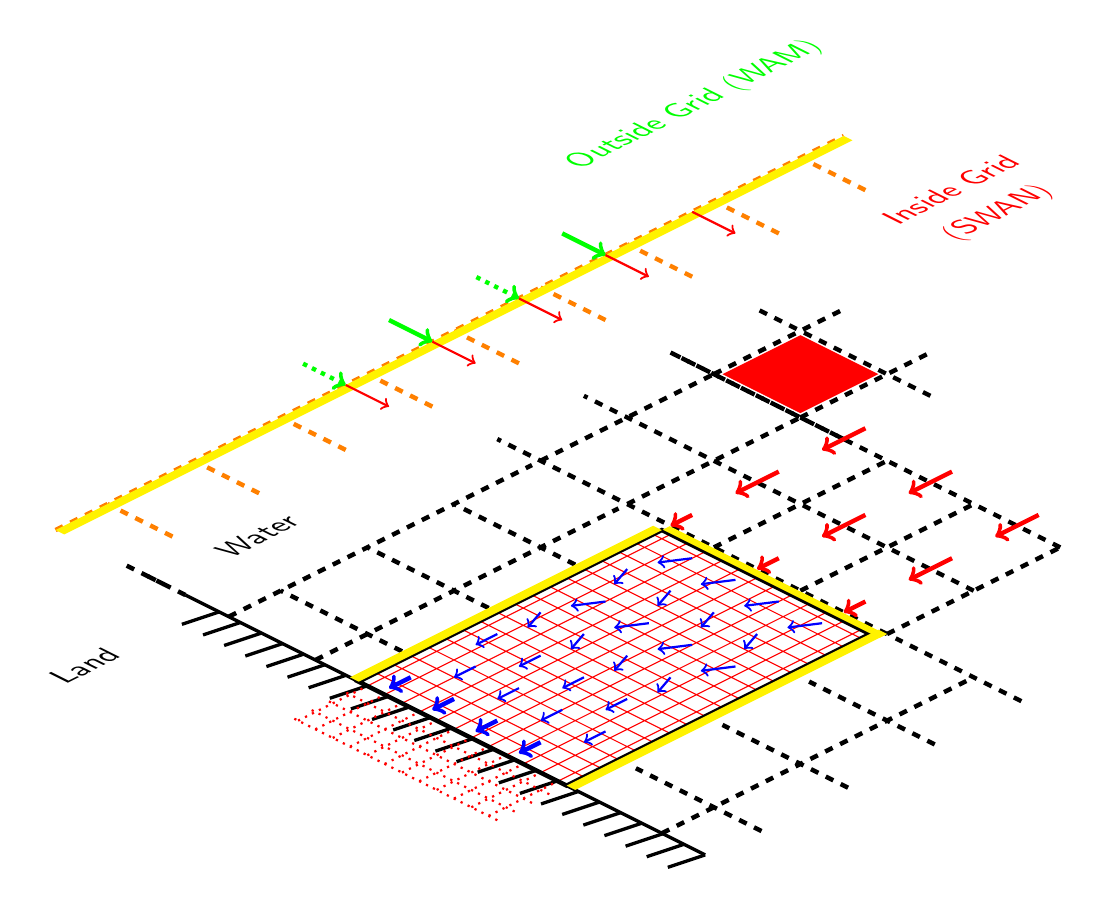
\begin{tikzpicture}[scale=.55,interface/.style={
	        postaction={draw,decorate,decoration={border,angle=45,
	                    amplitude=0.5cm,segment length=3mm}}}]
	
	
		\begin{scope}[xshift=-100mm,
		yshift=90,every node/.append style={
		yslant=0.5,xslant=-1},yslant=0.5,xslant=-1
		             ]
		%\fill[white,fill opacity=.9] (0,0) rectangle (7,9);
	%Coarse grid is obtained by drawins subgridS and puzzling them together. 
	
	\draw[step=20mm,black,ultra thick,dashed] (2,0) grid (6,9); 
	\draw[step=20mm,black,ultra thick,dashed] (6,5) grid (9,9); 
	%interface
	\draw[line width=.8pt,interface,very thick,black](-5.2,-3)--(-5.2,9);
	%nested grid
	\draw[step=4mm, red] (-5.2,.2) grid (1.8,5);
	\draw[step=4mm, thick,red,dotted] (-6.8,.2) grid (-5.2,5);
	\draw[black,ultra thick] (-5.2,.2) rectangle (1.8,5);
	
	\draw[step=20mm,black,ultra thick,dashed] (-5.2,-.2) grid (2,-3.1);%XXXXXX
	\draw[step=20mm,black,ultra thick,dashed] (-5.2,5.2) grid (1.8,8); 
	
	%filling
	\fill[yellow,ultra thick] (1.82,0) rectangle (1.98,5);%boundary area
	\fill[yellow,ultra thick] (-5.2,5) rectangle (1.8,5.2);%boundary area
	\fill[yellow,ultra thick] (-5.2,.2) rectangle (2,0);%boundary area
	\fill[red,ultra thick] (6.1,6.1) rectangle (7.9,7.9);%cell element
	%	%axes
	%	\draw[->,very thick,black](-3,-5) to[](-2,-5);
	%	\draw[->,very thick,black](-3,-5) to[](-3,-4);
		%\draw[-,ultra thin,black,dashed](-4.5,-5) to[](-4.5,6);
	
	
	\draw[<-,ultra thick,black,red](3.5,1) to[](4.5,1);
	\draw[<-,ultra thick,black,red](3.5,3) to[](4.5,3);
	\draw[<-,ultra thick,black,red](3.5,5) to[](4.5,5);
	
	\draw[<-,ultra thick,black,red](2,1) to[](2.5,1);
	\draw[<-,ultra thick,black,red](2,3) to[](2.5,3);
	\draw[<-,ultra thick,black,red](2,5) to[](2.5,5);
	%arrows interacting with yellow boundary zone
	\draw[<-,ultra thick,black,red](5.5,1) to[](6.5,1);
	\draw[<-,ultra thick,black,red](5.5,3) to[](6.5,3);
	\draw[<-,ultra thick,black,red](5.5,5) to[](6.5,5);
	%Inside the grid
%	\foreach \t in {-80,-60,...,80} { \DrawLatitudeCircle[\R]{\t} }

	%\foreach \y in {0.5,1,...,3} { \draw[<-](1,{\y}) to[](1.5,{\y})};
	\draw[<-,ultra thick,blue](-5,1.5) to[](-4.5,1.5);
	\draw[<-,ultra thick,blue](-5,2.5) to[](-4.5,2.5);
	\draw[<-,ultra thick,blue](-5,3.5) to[](-4.5,3.5);
	\draw[<-,ultra thick,blue](-5,4.5) to[](-4.5,4.5);

	
	
	\draw[<-,thick,blue](-4,1) to[](-3.5,1);
	\draw[<-,thick,blue](-4,2) to[](-3.5,2);
	\draw[<-,thick,blue](-4,3) to[](-3.5,3);
	\draw[<-,thick,blue](-4,4) to[](-3.5,4);
  
  \draw[<-,thick,blue](-3,1.5) to[](-2.5,1.5);
	\draw[<-,thick,blue](-3,2.5) to[](-2.5,2.5);
	\draw[<-,thick,blue](-3,3.5) to[](-2.5,3.5);
	\draw[<-,thick,blue](-3,4.5) to[](-2.5,4.5);



  \draw[<-,thick,blue](-2,1.3) to[](-1.5,1.5);
	\draw[<-,thick,blue](-2,2.3) to[](-1.5,2.5);
	\draw[<-,thick,blue](-2,3.3) to[](-1.5,3.5);
	\draw[<-,thick,blue](-2,4.3) to[](-1.5,4.5);


  \draw[<-,thick,blue](-1,1.3) to[](-.5,1);
	\draw[<-,thick,blue](-1,2.3) to[](-.5,2);
	\draw[<-,thick,blue](-1,3.3) to[](-.5,3);
	\draw[<-,thick,blue](-1,4.3) to[](-.5,4);



  \draw[<-,thick,blue](0,1.3) to[](.5,1.5);
	\draw[<-,thick,blue](0,2.3) to[](.5,2.5);
	\draw[<-,thick,blue](0,3.3) to[](.5,3.5);
	\draw[<-,thick,blue](0,4.3) to[](.5,4.5);


  \draw[<-,thick,blue](1,1.3) to[](1.5,1);
	\draw[<-,thick,blue](1,2.3) to[](1.5,2);
	\draw[<-,thick,blue](1,3.3) to[](1.5,3);
	\draw[<-,thick,blue](1,4.3) to[](1.5,4);


	%\draw[<-,thick,blue](-4,5) to[](-3.5,5);
%  \draw[<-,ultra thick,black,green](1,3) to[](1.5,3);	
	%WAM or WAVEWATCH forcing
	\draw[-,ultra thick,dashed, black] (-5.2,9) to[] (-5.2,10);
		\draw[-,ultra thick,dashed, black] (-5.2,9.5) to[] (-5.2,10.5);
	\draw[-,step=20mm,ultra thick,dashed, orange] (-5.2,10.5) grid (13,12);
	\fill[yellow] (-5.2,11.8) rectangle (13,12);
	
  \draw[<-,ultra thick,green,dotted](1.5,12) to[](1.5,13);
	\draw[<-,ultra thick,green](3.5,12) to[](3.5,13);
	\draw[<-,ultra thick,green,dotted](5.5,12) to[](5.5,13);
	\draw[<-,ultra thick,green](7.5,12) to[](7.5,13);


  \draw[<-,thick,red](1.5,11) to[](1.5,12);
	\draw[<-,thick,red](3.5,11) to[](3.5,12);
	\draw[<-,thick,red](5.5,11) to[](5.5,12);
	\draw[<-,thick,red](7.5,11) to[](7.5,12);
	\draw[<-,thick,red](9.5,11) to[](9.5,12);


%pointers
  \draw[thick](-8,9)node[below]{$\mathsf{Land}$};
   \draw[thick](-3,10)node[below]{$\mathsf{Water}$};
\draw[thick,red](13,10)node[below]{$\mathsf{Inside\ Grid}$};
\draw[thick,green](12,15)node[below]{$\mathsf{Outside\ Grid\ (WAM)}$};
\draw[thick,red](13,9)node[below]{$\mathsf{(SWAN)}$};


	\end{scope}
	
	
	
	
	\end{tikzpicture}
	\caption[Nested Grids in SWAN and WAM coupling]{SWAN nested (finer resolution) grid represented in red and computational grid (coarser) in black. On the former occours bla bla bla; grid covers land wich is assumed to totally absorb incoming spectral flux \textit{killing} back-propagation. On the latter bla bla bla. Boundary zone between grids drawn in yellow: note how incoming signal (outside yellow rectangle) duplicates or triplicates \textit{once crossed} boundary (inside yellow rectangle) for both cases. Same principle holds for nesting with WAM whose incoming signal (green) has lower spatial resolution, which is improved once passed \textit{trough} the yellow interface. Note how resolution tend to increasem by approaching shallow waters. WAM/SWAN interface drawn in orange. Cell grid (red filled box), represented in Fig.(??)}
	\label{fig:nesting}
\end{figure}
\end{document}